% Appendices. Same mechanism as the template: \section titles typed as "Appendix X: ...", Roman section counter.
% This file starts the appendix numbering itself; if main.tex already does the same before \input, the repeats are harmless.
\setcounter{figure}{0}\setcounter{table}{0}
\renewcommand{\thefigure}{A.\arabic{figure}}
\renewcommand{\thetable}{E.\arabic{table}}

\section{Appendix A: Snapshots}
Figure~\ref{fig:appA-water-wet} shows two further review strips from the qualitative comparison on our own recordings (Section~\ref{sec:ch6-results}): a water-filled cavity and a wet patch, each processed by the earlier implementation, the baseline and the candidate, with the confidence of each box drawn on the frame. The frames were picked by hand, include cases unfavourable to each model, and are not representative. There is no ground truth for these recordings.

\begin{figure}[H]
\centering
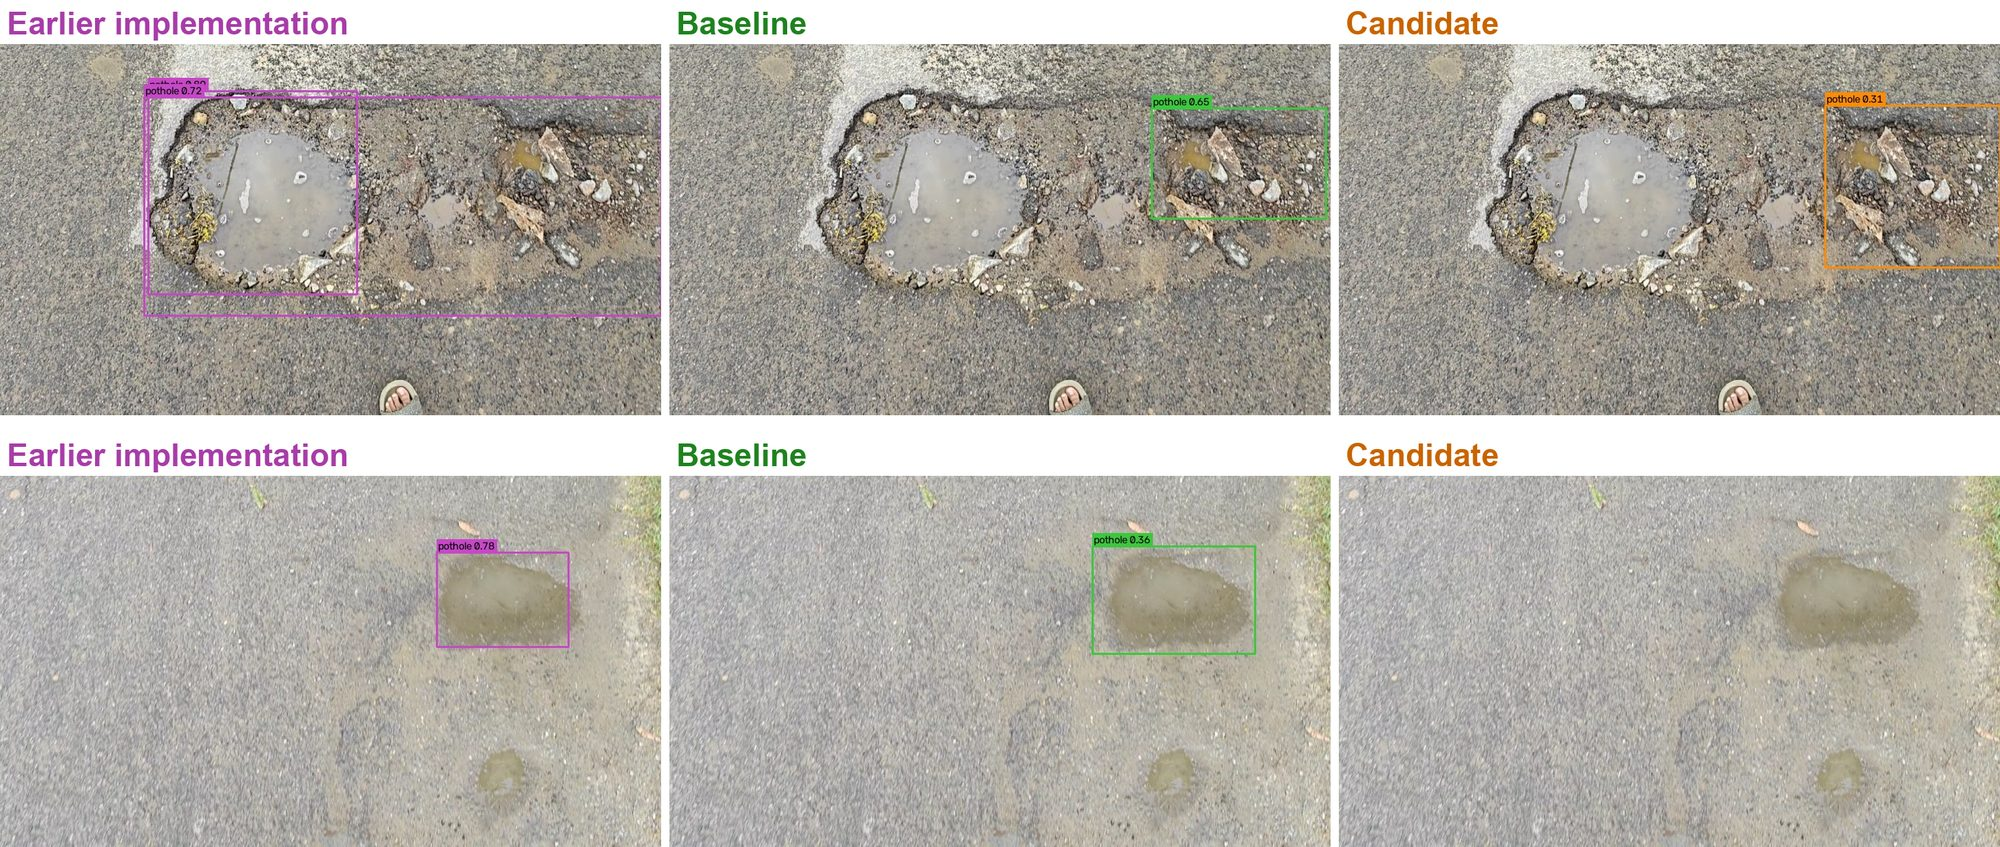
\includegraphics[width=\textwidth]{appA_strips_water_wet.jpg}
\caption{Review strips (hand-picked, not representative): a water-filled cavity (top) and a wet patch (bottom), processed by the earlier implementation, the baseline and the candidate. These frames have no ground-truth labels, so the view is qualitative.}
\label{fig:appA-water-wet}
\end{figure}

% OUTSTANDING: screenshots of the web interface (dashboard, upload, sessions, detections, route planner)
% do not exist yet. Add them here as figures appA_<name>.png when captured.
\clearpage

\section{Appendix B: Details of list of publications related to this project}
\begin{table}[H]
\centering
\renewcommand{\arraystretch}{1.3}
\begin{tabular}{|p{4.6cm}|p{8.6cm}|}
\hline
\textbf{Item} & \textbf{Details} \\
\hline
Author names & Zain Mahedi, Thanu George, Vikas Shashi, Tanish Agrawal (under the guidance of Dr. Seema Patil) \\
\hline
Paper title & AI Powered Pothole Detection and Intelligent Route Optimization System \\
\hline
Name of the conference or journal & 2nd International Conference on Emerging Technologies in Computer Science for Interdisciplinary Applications (Track: Artificial Intelligence and Machine Learning) \\
\hline
Paper ID & 722 \\
\hline
Submission status & Submitted on 30 September 2026 through Microsoft CMT; under review \\
\hline
Place of the conference & To be announced \\
\hline
Date of the conference & To be announced \\
\hline
\end{tabular}
\caption*{Publication submitted by the team. No acceptance has been received.}
\end{table}

The submission describes the earlier phase of this work, the earlier implementation described in Chapter~\ref{ch:intro}, and not the rebuilt system reported here.
\clearpage

\section{Appendix C: Details of Patent}
% No entry. The Phase 1 report left this appendix empty; the team should fill it in or state "Nil".
\clearpage

\section{Appendix D: Details of Funding}
% No entry. The Phase 1 report left this appendix empty; the team should fill it in or state "Nil".
\clearpage

\section{Appendix E: POs and PSOs Mapped}
\setcounter{table}{0}
Each justification below refers to work carried out in the rebuilt system.
% OUTSTANDING: the levels are copied from the Phase 1 report and must be confirmed by the team.

\begin{table}[H]
\centering
\setstretch{1}
\footnotesize
\renewcommand{\arraystretch}{1.1}
\setlength{\tabcolsep}{5pt}
\begin{tabular}{|p{2.7cm}|c|p{8.9cm}|}
\hline
\textbf{PROGRAMME OUTCOMES} & \textbf{Level (1/2/3)} & \textbf{Justification if addressed} \\
\hline
PO1 & 3 & Applies mathematics, statistics, machine learning and geospatial computation: detection metrics and bootstrap intervals, perceptual-hash grouping of images, and a shortest-path route cost on a road graph. \\
\hline
PO2 & 3 & Analyses the shortcomings of the earlier implementation and of the public datasets (leakage between splits, label noise, domain gap) and formulates a single-class box detection problem with a leakage-controlled evaluation. \\
\hline
PO3 & 3 & Designs the complete system: dataset pipeline, detector, tracker, de-duplication of sightings, map matching, route planner, REST API, database and browser interface. \\
\hline
PO4 & 3 & Conducts experiments with group-aware splits, validation-selected thresholds, group-bootstrap intervals and paired comparisons, and reports a negative result for the candidate model. \\
\hline
PO5 & 3 & Uses PyTorch, Ultralytics YOLOv8, OpenCV, FastAPI, SQLite, OSMnx, NetworkX, Leaflet and pytest, and a rented cloud GPU for training. \\
\hline
PO6 & 3 & Addresses road safety by detecting and mapping potholes and by planning routes that account for them; the route comparison is demonstrated on a synthetic session only. \\
\hline
PO7 & 2 & Supports sustainable infrastructure maintenance through data-driven road monitoring from ordinary forward-facing phone or dashcam video and open map data. \\
\hline
PO8 & 2 & Follows ethical practice by using public datasets under their stated licences, flagging licences that were not verified, processing video and location data on the user's own machine, and reporting limitations, the automated review of labels and the negative result openly. \\
\hline
PO9 & 3 & The work was carried out by a team of four under the guidance of the project guide, with the work divided among data preparation, model training and evaluation, application development and testing. \\
\hline
PO10 & 2 & Communicates the work through this report, the project documentation (design decisions, API reference, dataset audit notes) and the browser interface. \\
\hline
PO11 & 2 & Plans the work in phases and keeps cost low through open-source software, public datasets, existing hardware and about \$0.77 of rented GPU time for the candidate training run. \\
\hline
PO12 & 2 & Involves learning new techniques (perceptual hashing, group-bootstrap evaluation, cloud GPU workflow, graph routing) and identifies directions for further work in Chapter~\ref{ch:conclusion}. \\
\hline
\end{tabular}
\caption{Programme Outcomes Mapping with Project}
\end{table}

\begin{table}[H]
\centering
\setstretch{1}
\small
\renewcommand{\arraystretch}{1.3}
\setlength{\tabcolsep}{5pt}
\begin{tabular}{|p{2.7cm}|c|p{8.9cm}|}
\hline
\textbf{PROGRAMME SPECIFIC OUTCOMES} & \textbf{Level (1/2/3)} & \textbf{Justification if addressed} \\
\hline
PSO1 & 2 & Implements a client-server system: a browser client calls a FastAPI REST API with background job processing and SQLite storage on the server. \\
\hline
PSO2 & 3 & Applies software engineering practice (a modular package, validated configuration, 1,101 automated tests, recorded hashes and configurations for reproducible training runs) and machine learning to a real-world problem. \\
\hline
PSO3 & 3 & Integrates computer vision, geospatial data and web technology into one system for road monitoring and route recommendation, demonstrated on recorded video and a synthetic route session. \\
\hline
\end{tabular}
\caption{Programme Specific Outcomes Mapping with Project}
\end{table}
\clearpage

\section{Appendix F: Similarity report, AI Generated report}
\setcounter{figure}{0}\renewcommand{\thefigure}{F.\arabic{figure}}
The report text was checked with Turnitin. Figure~\ref{fig:appF-similarity} shows the similarity summary and Figure~\ref{fig:appF-ai} the AI writing detection summary.

\begin{figure}[H]
\centering
\fbox{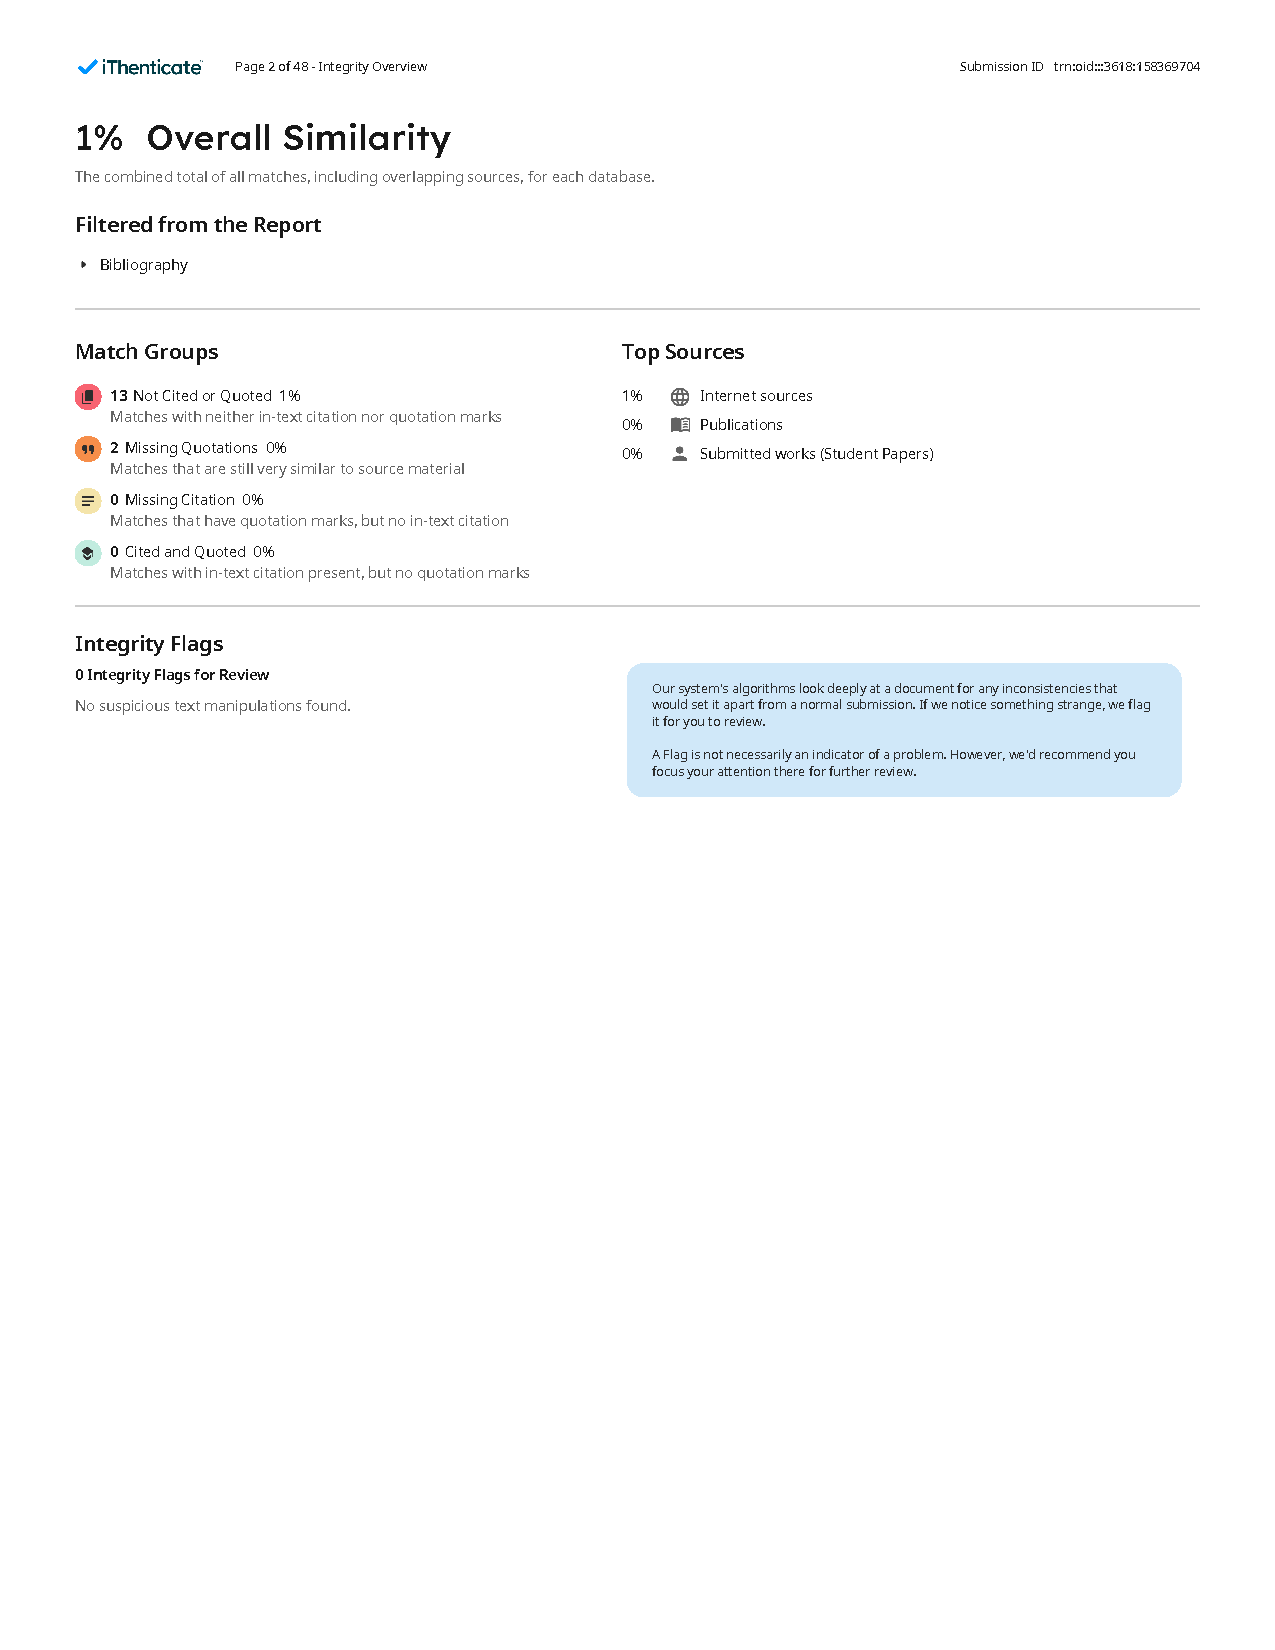
\includegraphics[width=0.97\textwidth]{appF_similarity_report.pdf}}
\caption{Turnitin similarity report summary.}
\label{fig:appF-similarity}
\end{figure}

\begin{figure}[H]
\centering
\fbox{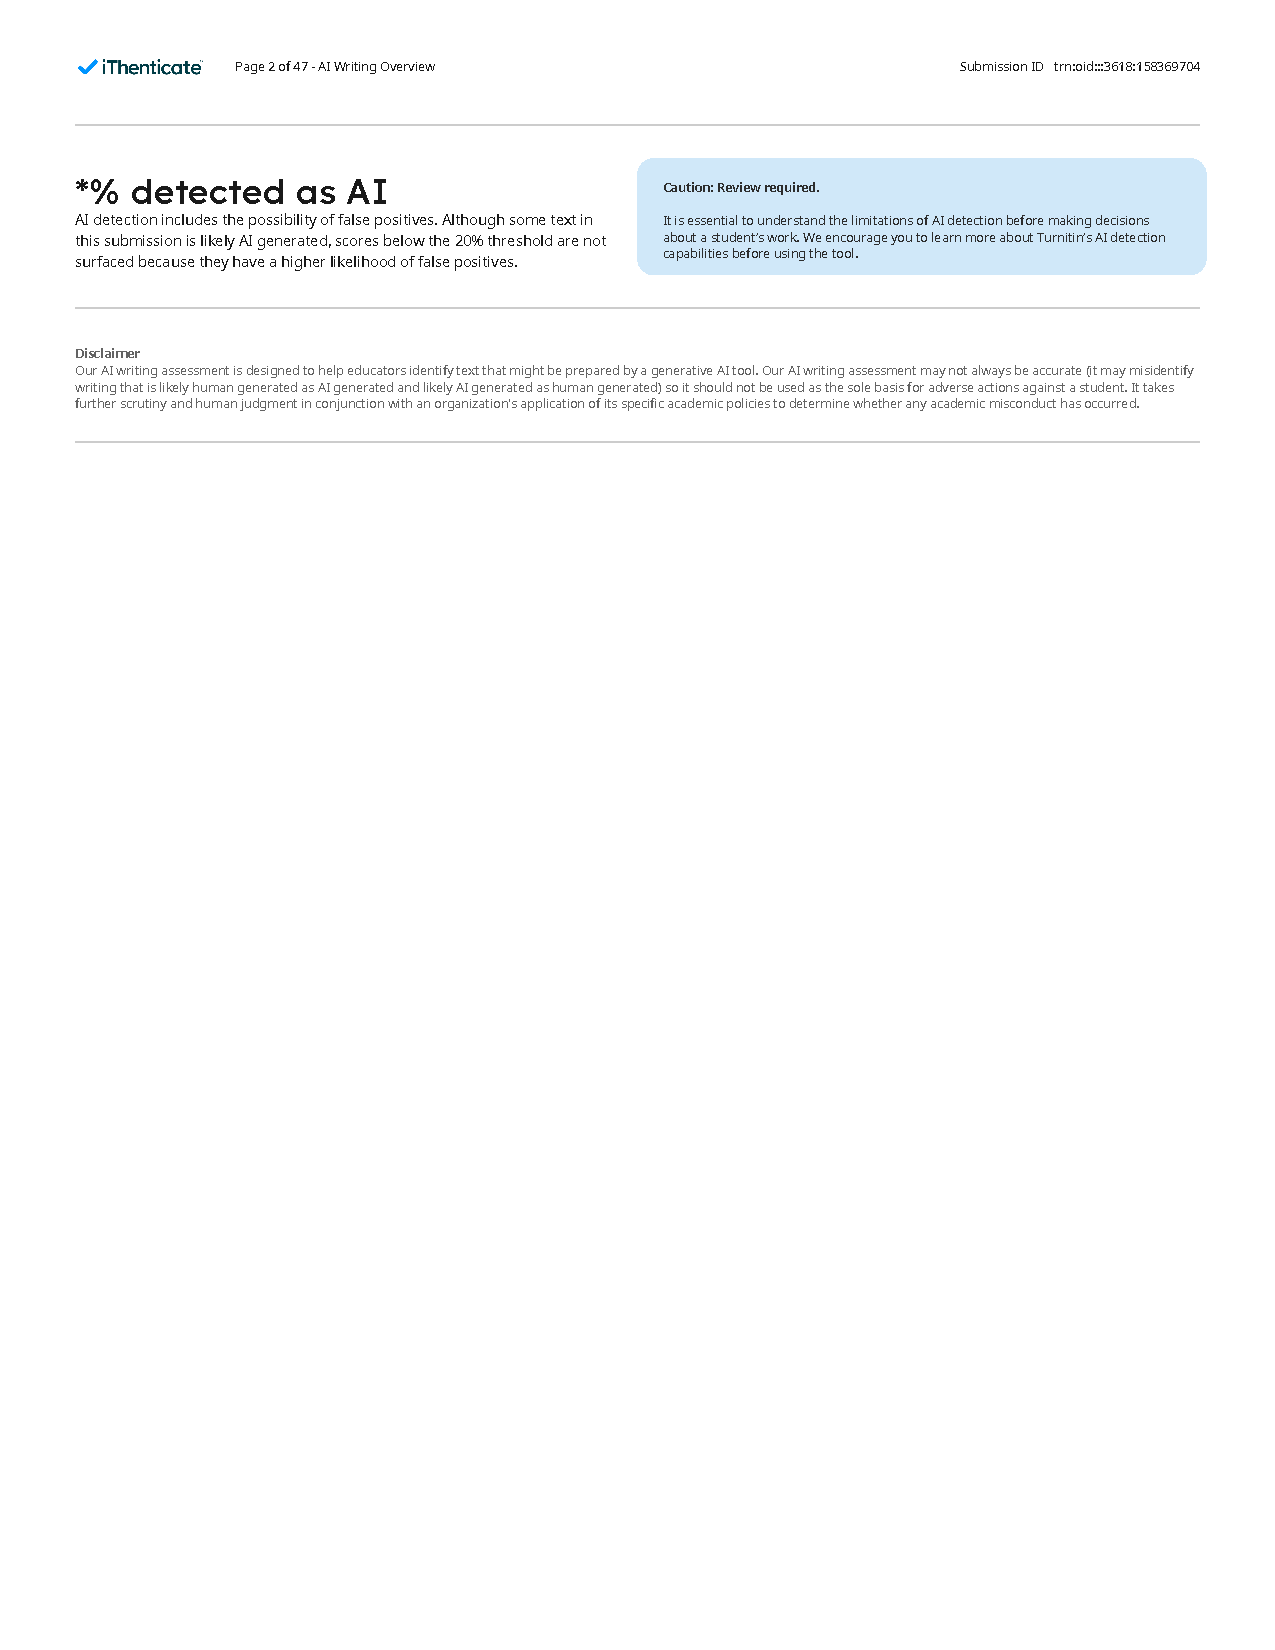
\includegraphics[width=0.97\textwidth]{appF_ai_report.pdf}}
\caption{Turnitin AI writing detection summary.}
\label{fig:appF-ai}
\end{figure}
\clearpage
